%%
%% ASE 2026 paper, ACM sigconf template
%%
\documentclass[sigconf,anonymous]{acmart}

%% Packages
\usepackage{algorithmic}
\usepackage{graphicx}
\usepackage{textcomp}
\usepackage{xcolor}
\usepackage{enumitem}
\usepackage{multirow}
\usepackage{tabularx}
\usepackage{array}
\usepackage{booktabs}
\usepackage{siunitx}
\usepackage{subcaption}
\usepackage{adjustbox}
\usepackage{dblfloatfix}
\setlength{\emergencystretch}{2em}

%% \BibTeX command to typeset BibTeX logo in the docs
\AtBeginDocument{%
  \providecommand\BibTeX{{%
    Bib\TeX}}}

%% Suppress copyright/reference blocks for submission stage
\setcopyright{none}
\settopmatter{printacmref=false}
\renewcommand\footnotetextcopyrightpermission[1]{}
\pagestyle{plain}

%%
%% The document starts here
%%
\begin{document}

%%
%% Title and author information
%%
\title{Unravel: Root-Cause Analysis of RISC-V Build Failures via Long-Range Evidence Extraction and Rule-Tree Reasoning}

%% ---- Authors (hidden for anonymous submission) ----
%\author{Zehua Wang}
%\affiliation{%
%  \institution{Institute of Software, Chinese Academy of Sciences}
%  \city{Beijing}\country{China}}
%\email{wangzehua23@otcaix.iscas.ac.cn}
%
%\author{Zhirou Ma}
%\affiliation{%
%  \institution{Institute of Software, Chinese Academy of Sciences}
%  \city{Beijing}\country{China}}
%\email{mazhirou@otcaix.iscas.ac.cn}
%
%\author{Jie Liu}
%\authornote{Corresponding author}
%\affiliation{%
%  \institution{Institute of Software, Chinese Academy of Sciences}
%  \city{Beijing}\country{China}}
%\email{ljie@otcaix.iscas.ac.cn}
%
%\author{Liangyi Kang}
%\affiliation{%
%  \institution{Institute of Software, Chinese Academy of Sciences}
%  \city{Beijing}\country{China}}
%\email{kangliangyi15@otcaix.iscas.ac.cn}
%
%\author{Shuai Wang}
%\affiliation{%
%  \institution{Institute of Software, Chinese Academy of Sciences}
%  \city{Beijing}\country{China}}
%\email{wangshuai@otcaix.iscas.ac.cn}
%
%\author{Dan Ye}
%\authornote{Corresponding author}
%\affiliation{%
%  \institution{Institute of Software, Chinese Academy of Sciences}
%  \city{Beijing}\country{China}}
%\email{yedan@otcaix.iscas.ac.cn}
%
%\author{Jiaxin Zhu}
%\affiliation{%
%  \institution{Institute of Software, Chinese Academy of Sciences}
%  \city{Beijing}\country{China}}
%\email{zhujiaxin@otcaix.iscas.ac.cn}
%
%\author{Wei Wang}
%\affiliation{%
%  \institution{Institute of Software, Chinese Academy of Sciences}
%  \city{Beijing}\country{China}}
%\email{wangwei@otcaix.iscas.ac.cn}
%
%\author{Hua Zhong}
%\affiliation{%
%  \institution{Institute of Software, Chinese Academy of Sciences}
%  \city{Beijing}\country{China}}
%\email{zhonghua@otcaix.iscas.ac.cn}
%
%\renewcommand{\shortauthors}{Wang et al.}

%% Funding acknowledgments (hidden for submission)
%\thanks{Supported by Strategic Priority Research Program of the Chinese Academy of Sciences (XDA0320102), the National Natural Science Foundation of China (42361144884)}

%% Conference information
\acmConference[ASE '26]{2026 41st IEEE/ACM International Conference on Automated Software Engineering}{October 12--16, 2026}{Munich, Germany}
\acmYear{2026}

%%
%% Abstract
%%
\begin{abstract}
Porting software to RISC-V triggers build failures whose root causes are buried in ultra-long logs. Two challenges impede automation: (C1)~failure clues constitute fewer than 5\% of log content and may appear hundreds of lines before the terminal error, creating long-range causal dependencies that naive truncation breaks; (C2)~superficially similar errors may require different fixes depending on build stage and toolchain context, making similarity-based retrieval unreliable. We propose \textbf{Unravel}, a two-stage framework. Stage-1 (\emph{Long-Range Evidence Extraction}) combines error-anchor localization, entity-guided backtracking, and semantic summarization to preserve evidence chains under strict token budgets. Stage-2 (\emph{Rule-Tree Reasoning}) distills repair rules from historical commits into a condition-aware tree index and applies iterative evidence-driven routing for traceable diagnosis. On 127 real RISC-V failures from a production OBS, Stage-1 improves recall and F1 over the strongest baseline by 15.5\% and 3.7\%; the full pipeline achieves an expert-rated diagnostic score of 84.0\%, outperforming MCTS by 8.7\% with~61\% less processing time.
\end{abstract}

%%
%% Keywords
%%
\keywords{RISC-V, build failure, root cause analysis, critical error extraction, large language model}

%% CCS Concepts (required by ACM)
\begin{CCSXML}
<ccs2012>
<concept>
<concept_id>10011007.10011074.10011099.10011102.10011103</concept_id>
<concept_desc>Software and its engineering~Software testing and debugging</concept_desc>
<concept_significance>500</concept_significance>
</concept>
<concept>
<concept_id>10011007.10011074.10011099.10011102.10011104</concept_id>
<concept_desc>Software and its engineering~Software maintenance tools</concept_desc>
<concept_significance>300</concept_significance>
</concept>
</ccs2012>
\end{CCSXML}

\ccsdesc[500]{Software and its engineering~Software testing and debugging}
\ccsdesc[300]{Software and its engineering~Software maintenance tools}

%%
%% Make title
%%
\maketitle

%% ===== Section 1 Introduction =====
\section{Introduction}

RISC-V has gained significant momentum in recent years, driven by its open instruction-set architecture, modularity, and extensibility~\cite{cui2023risc}, positioning it as a compelling alternative for next-generation general-purpose and domain-specific computing. As software migration advances, two practical realities have become increasingly clear. First, the number of failed packages is large in real migration workflows: large-scale CI studies report 34,182 failed builds across 767 projects (349 OSS projects and 418 projects in a financial organization)~\cite{vassallo2017tale}. Second, migration is not a one-shot process. Even after a package is repaired once, upstream version changes, dependency updates, and toolchain evolution can re-trigger failures in later cycles~\cite{lou2020understanding}. In engineering practice, handling such recurring failures still relies heavily on manual root-cause analysis from build logs before developers can apply reliable fixes.

Compared with native builds on established architectures, RISC-V cross-compilation further compounds these difficulties. Cross-toolchains introduce additional build stages---host/target toolchain probing, architecture-feature detection, and QEMU-based test execution---that lengthen logs and widen the distance between triggering conditions and observable errors. In our dataset, RISC-V build logs average 1{,}175 lines per failure. Moreover, a single error message such as \texttt{undefined reference} may originate from architecture-specific causes (e.g., missing RISC-V vector intrinsics) or from generic causes (e.g., an outdated library version), yet the required fixes differ fundamentally: one demands conditional assembly patches while the other requires a dependency version bump. This architecture-generic ambiguity, combined with the expanded build-stage pipeline, makes RISC-V migration a particularly challenging setting for automated diagnosis.

\begin{figure*}[!tb]
    \centering
    \begin{subfigure}[t]{0.48\textwidth}
        \centering
        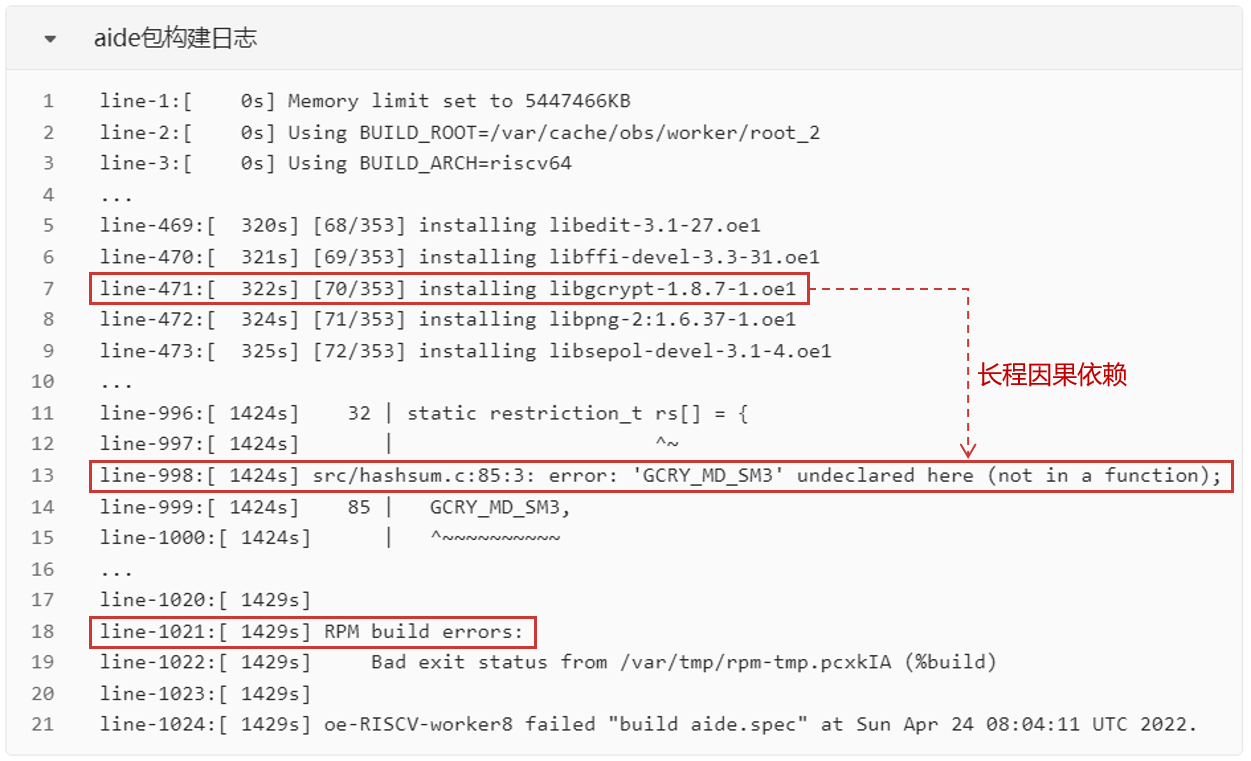
\includegraphics[width=\textwidth]{pic/log-causal-dependency.png}
        \caption{Long-range causal dependencies in build logs}
        \label{fig:causal-dep}
    \end{subfigure}
    \hfill
    \begin{subfigure}[t]{0.48\textwidth}
        \centering
        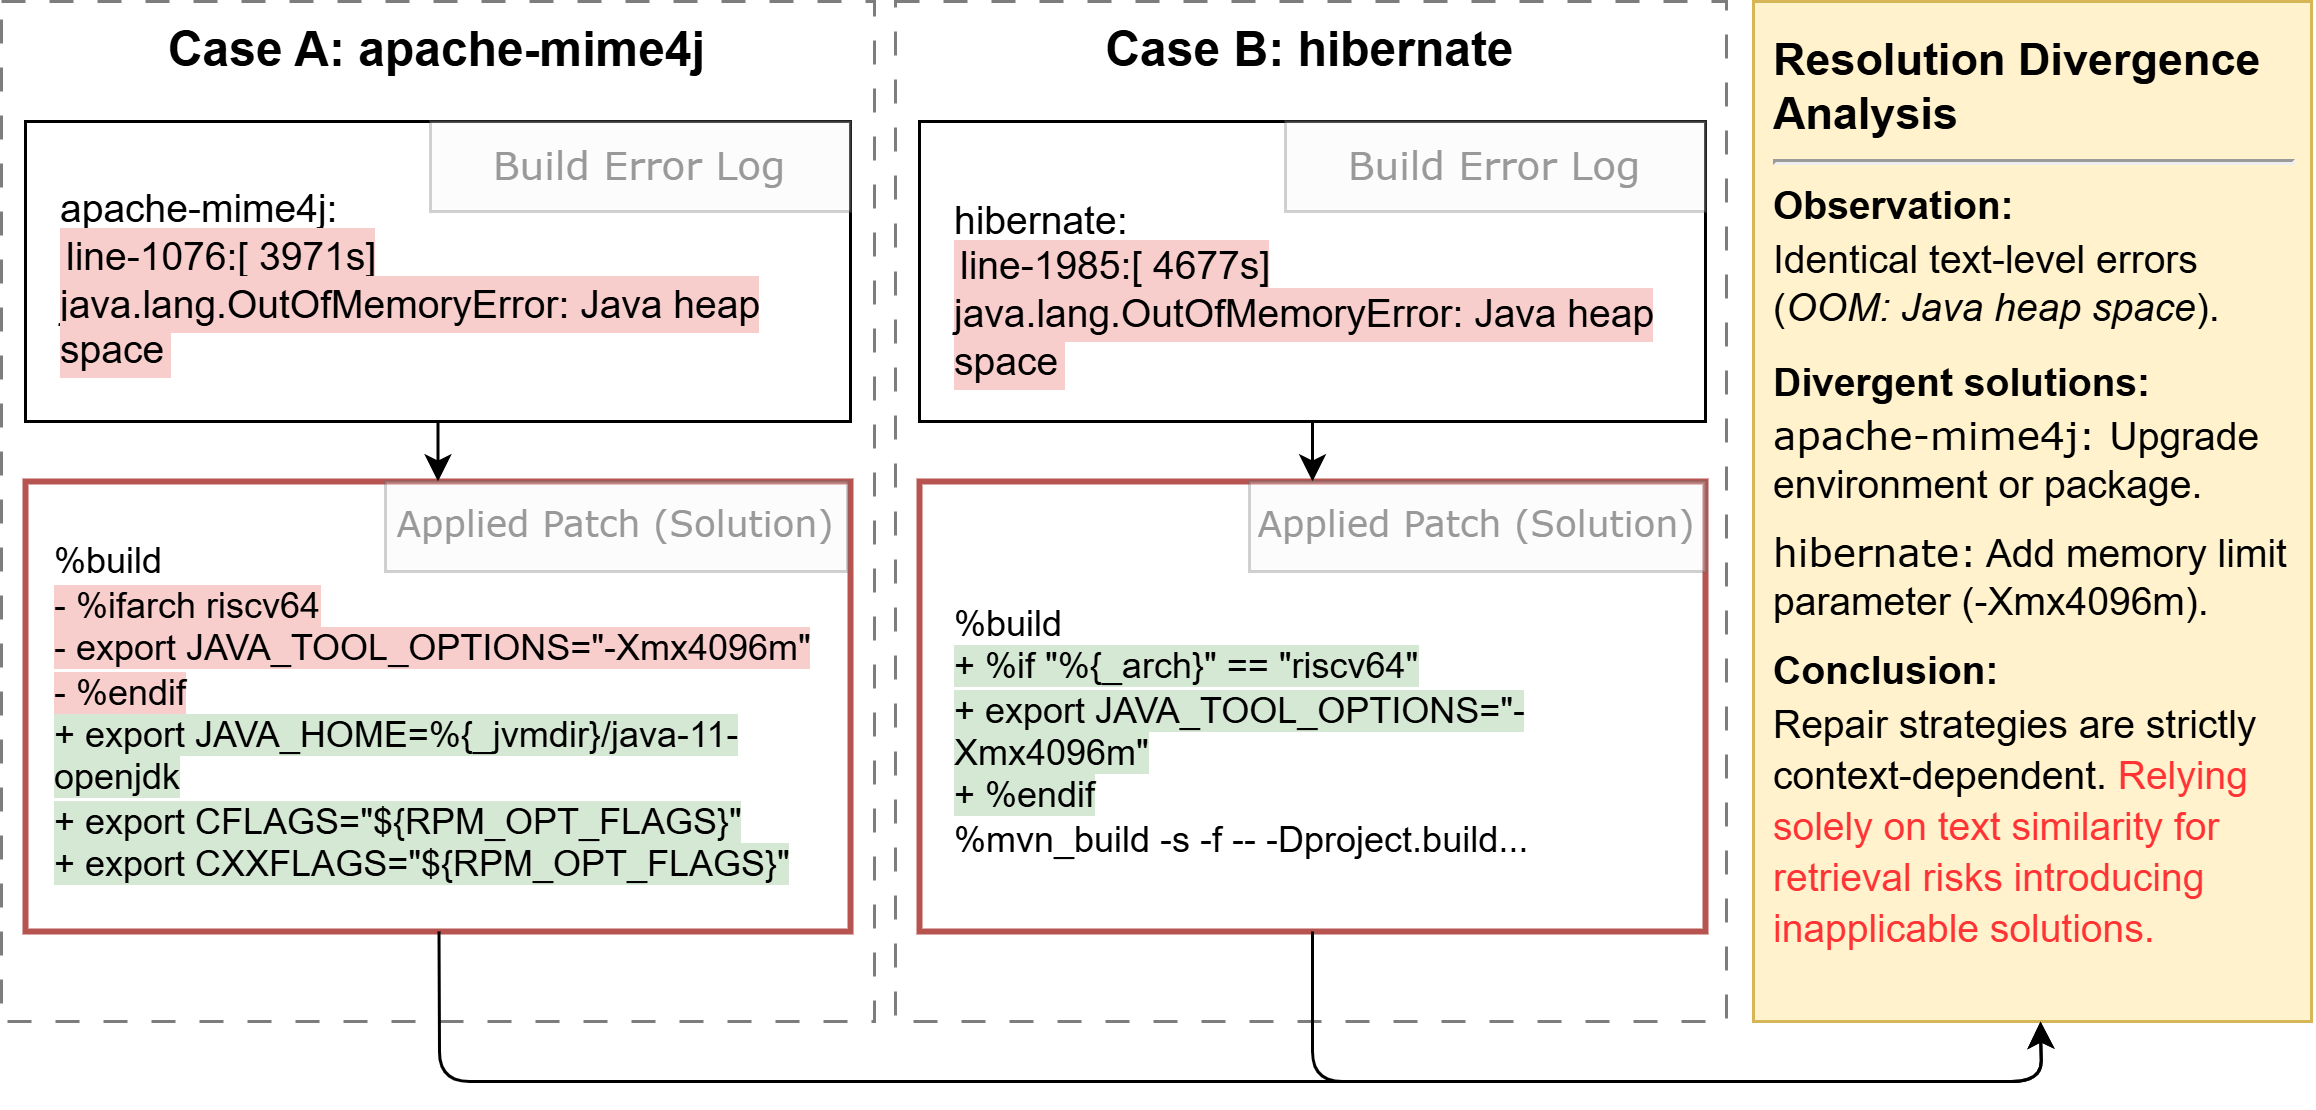
\includegraphics[width=\textwidth]{pic/similar-misleading.png}
        \caption{Similar errors but different fixes}
        \label{fig:similar-mislead}
    \end{subfigure}
    \caption{Motivating examples. (a) A build log with long-range causal dependency: the root cause at line 471 is far from the error at line 998. (b) Similarity misleading: two packages share the same error message but require different fixes.}
    \Description{Left: a build log snippet showing three highlighted regions illustrating long-range causal dependencies. Right: two build-log excerpts sharing the same error message but requiring different repair actions.}
\end{figure*}

RISC-V build logs also expose two core technical difficulties. \textbf{Problem 1: long-range causal dependency in ultra-long logs.} Figure~\ref{fig:causal-dep} shows a representative failure from \texttt{aide}: the build terminates with a generic \texttt{RPM build errors} signal near the tail (line 1021), and an explicit compile-time symptom appears at line 998 (\texttt{`GCRY\_MD\_SM3' undeclared}). However, the actual trigger is much earlier (line 471), where the dependency installation step introduces \texttt{libgcrypt-1.8.7-1.oe1}, whose feature set does not provide SM3 support. This head--middle--tail separation means that root-cause evidence is distributed across distant regions and different build phases. If diagnosis keeps only a local window around the explicit error line, the decisive dependency-version clue is likely to be removed.

\textbf{Problem 2: similarity misleading across failure cases.} Figure~\ref{fig:similar-mislead} presents two logs (\texttt{apache-mime4j} and \texttt{hibernate}) that contain highly similar surface-level error messages, but their actionable causes differ. One case is rooted in package/dependency adaptation, while the other is tied to build-script and environment constraints; consequently, applying the same fix template to both cases leads to incorrect remediation in at least one of them. This example shows that successful repair depends not only on error text matching, but also on applicability conditions such as build stage, dependency state, architecture constraints, and toolchain configuration.

These issues make manual diagnosis costly and slow. Large language models (LLMs) have recently opened a new opportunity for automating build-failure diagnosis, but directly applying LLMs still faces two major challenges: \textbf{(C1)} build logs are often much longer than practical context budgets, and naive truncation breaks evidence chains; \textbf{(C2)} LLMs lack specialized RISC-V build knowledge and cannot reliably distinguish architecture-specific from generic failure causes, while vector-similarity-based RAG can introduce misleading historical cases when applicability conditions are not explicitly modeled. Recent LLM-agent frameworks~\cite{wang2024rcagent,yang2024swe} mitigate single-turn limitations through iterative tool use, yet they treat the underlying knowledge as a flat retrieval corpus and leave the core extraction and knowledge-organization challenges unaddressed.

To address these challenges, we propose \textbf{Unravel}, a unified framework with two tightly coupled stages. This paper makes the following contributions:
\begin{enumerate}[topsep=2pt,itemsep=3pt]
\item \textbf{Long-Range Evidence Extraction} (addressing C1). We design a multi-granularity extraction pipeline that combines error-anchor localization, entity-guided cross-stage backtracking, and lightweight semantic summarization to preserve high-fidelity evidence chains under strict token budgets. Stage-1 improves recall and F1 over the strongest baseline by 15.5\% and 3.7\%, respectively.
\item \textbf{Rule-Tree Reasoning} (addressing C2). We structure historical repair knowledge into condition-aware rules organized in a tree index by error type and build stage, and apply iterative conditional routing with domain-constrained tool invocation for traceable, evidence-grounded diagnosis. The full pipeline reaches a diagnostic score of 84.0\%, outperforming MCTS by 8.7\% with about 61\% less processing time.
\item \textbf{Empirical evaluation.} We evaluate Unravel on 127 real RISC-V build failures from a production OBS environment with four research questions covering extraction effectiveness, ablation, diagnostic quality, and efficiency, and deploy it in an industrial toolset plugin for practical RISC-V migration support.
\end{enumerate}

%% ===== Section 2 Related Work =====
\section{Related Work}

\subsection{Log Parsing and Build-Log Evidence Extraction}

Log parsing seeks to transform unstructured log data into structured representations. Classical approaches range from rule-based clustering~\cite{vaarandi2008mining} and tree-based online parsing~\cite{he2017drain} to $n$-gram dictionary methods~\cite{dai2020logram}. Deep learning methods learn temporal or semantic patterns for anomaly detection~\cite{du2017deeplog,guo2021logbert,chen2022bert,yang2021plelog}, and LLM-based approaches have further advanced this line with few-shot prompting~\cite{liu2024logprompt}, in-context learning~\cite{xu2024divlog}, and direct generative parsing~\cite{qi2023loggpt,guan2024logllm,ma2024llmparser}. For long-log scenarios, LogShrink~\cite{li2024logshrink} compresses logs by identifying commonality and variability patterns, and LogSage~\cite{xu2025logsage} proposes token-efficient preprocessing for CI/CD log analysis. However, these methods target general log parsing or anomaly detection; they do not address the task-specific challenge of preserving long-range causal evidence chains from build logs under strict context budgets~\cite{le2022log}.

From the build-failure perspective, prior empirical studies report frequent and diverse failures in CI and package-migration workflows~\cite{rausch2017empirical}, while recent engineering studies explore automatic build-error categorization to reduce manual triage effort~\cite{lee2024applying}. These efforts provide useful operational insights, but they still leave open the key challenge of extracting high-fidelity, long-range causal evidence from ultra-long build logs under strict context budgets.

\subsection{Log-based Root Cause Analysis}

Root cause analysis (RCA) seeks to identify the underlying causes of failures from system outputs. Traditional approaches employ rule-based correlation to match events~\cite{notaro2023logrule}, or combine log analysis with source-code examination to infer failing execution paths~\cite{yuan2010sherlog}. Deep learning methods formulate RCA as a log-line relevance ranking problem, extracting indicative descriptions and parameters from logs for structured diagnosis~\cite{wittkopp2024logrca}. Knowledge-based approaches organize failure patterns into structured representations: LogKG~\cite{sui2023logkg} constructs knowledge graphs from log events for structured diagnosis, and Squeeze~\cite{li2019generic} performs multi-dimensional root cause localization.

LLM-based RCA emphasizes generating human-readable diagnostic conclusions directly from failure logs. Roy et al.~\cite{roy2024exploring} demonstrate that agent-based designs can mitigate the sensitivity of single-turn question answering to context budgets and incomplete information. RCAgent~\cite{wang2024rcagent} further validates the effectiveness of tool-augmented LLMs for cloud-based RCA, and PACE-LM~\cite{zhang2023pace} explores calibrated confidence estimation with GPT-4 for incident analysis. A recent two-stage approach~\cite{shuai2025root} combines template-based key-evidence extraction with Monte Carlo tree search to guide LLM reasoning for RISC-V build failures. However, approaches that rely solely on ``similar-log retrieval + free-form generation'' risk introducing misleading evidence and amplifying hallucinations; applicability conditions, evidence alignment, and verification mechanisms must be systematically incorporated. Our method explicitly distills verifiable rules from historical repair experience and organizes them into a rule tree with conditional routing, thereby mitigating the risk of misleading retrieval at its source.

A parallel line of work designs autonomous agents for source-code bug repair. SWE-Agent~\cite{yang2024swe} navigates repository structures to localize and patch bugs, while Agentless~\cite{xia2024agentless} simplifies the pipeline with a two-phase localize-then-repair strategy. These systems operate on source code with full repository access, whereas build-failure RCA operates on build \emph{logs} without access to the failing codebase and targets diagnosis rather than patch generation, making the two lines complementary rather than directly comparable.

Despite this progress, no existing build-failure RCA method simultaneously addresses two key gaps: (1)~preserving long-range, cross-stage causal evidence under strict token budgets (most methods either truncate logs or rely on local windows), and (2)~explicitly modeling applicability conditions---such as build stage, dependency state, and target architecture---in historical repair knowledge (most retrieval-based methods match by surface similarity alone). These gaps motivate our framework design: preserving long-range evidence in Stage-1 and enforcing condition-aware, traceable rule-tree reasoning in Stage-2.

\begin{figure*}[!tb]
    \centering
    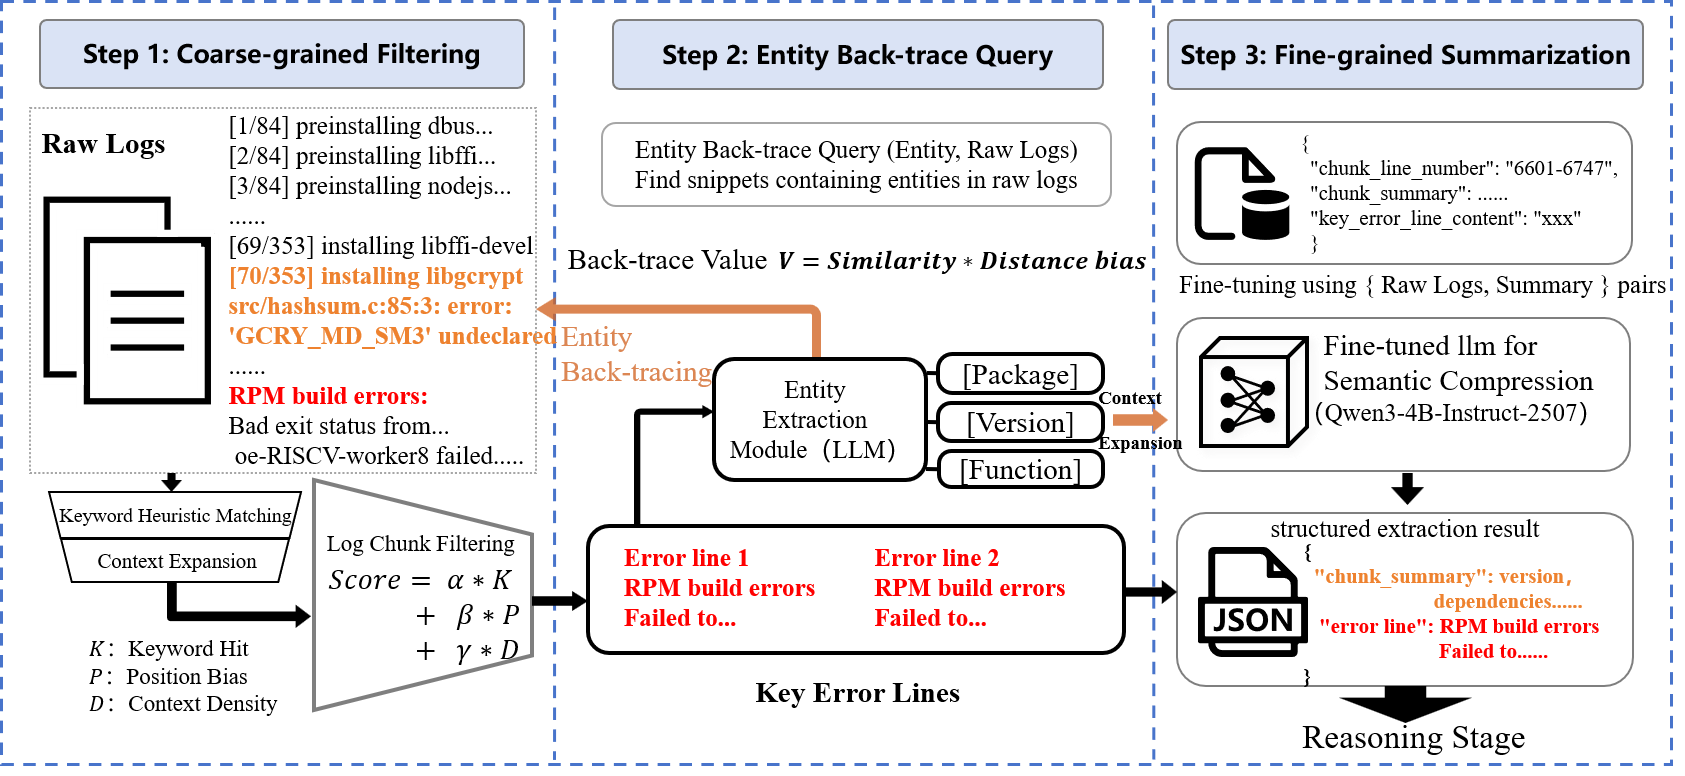
\includegraphics[width=\textwidth]{pic/mgsc-overview.png}
    \caption{Overall workflow of Unravel Stage-1: Long-Range Evidence Extraction from Build Logs}
    \Description{A three-step pipeline within Stage-1: Step-1 performs coarse-grained filtering with error anchor localization, Step-2 performs entity-based context backtracking, and Step-3 performs fine-grained semantic summarization.}
    \label{fig:mgsc}
\end{figure*}

%% ===== Section 3 Method =====
\section{Method}

A central observation motivating Unravel is that build-failure RCA decomposes into two structurally distinct sub-problems. The first---\emph{what happened}---requires identifying the causal evidence chain from ultra-long logs where fewer than 5\% of lines carry diagnostic value and key clues may be separated by hundreds of lines across build stages. The second---\emph{why it happened and how to fix it}---requires matching the observed failure against historical repair experience under verifiable preconditions, not surface-level text similarity. Existing approaches collapse both sub-problems into a single step: truncation-based prompting loses cross-stage evidence, while similarity-based retrieval ignores applicability conditions. Unravel separates these concerns into two tightly coupled stages: Stage-1 extracts high-fidelity evidence under a strict token budget, and Stage-2 performs condition-aware diagnosis over a rule-tree index. The two stages communicate through a structured summary $S$ whose fields---error anchors, entity traces, stage labels, and dependency states---are precisely the inputs that Stage-2 requires for conditional routing.

We emphasize that Unravel is \emph{not} a generic LLM-agent system applied to a new domain. Its core contributions lie in two domain-specific knowledge structures that existing agent frameworks lack. First, the multi-granularity extraction pipeline in Stage-1 (error-anchor localization, entity-guided backtracking, domain-tuned summarization) operates entirely without an LLM reasoning loop; it exploits the structured causal topology of build processes---where symbols, libraries, and macros serve as traceable cross-stage links---to recover evidence chains that no amount of iterative prompting can reconstruct from truncated inputs. Second, the rule-tree index in Stage-2 pre-materializes the diagnostic decision path of domain experts (error type $\to$ build stage $\to$ verifiable conditions $\to$ fix actions) as a routable knowledge structure with explicit applicability constraints, rather than storing experience as flat documents for similarity retrieval. The iterative reasoning loop in Stage-2 is deliberately minimal---limited to three domain-constrained tools---and serves only as the final inference interface over these pre-built structures. In short, the novelty resides in \emph{what} knowledge is extracted and \emph{how} it is organized, not in the agent loop itself.

\subsection{Extraction Stage: Long-Range Evidence Extraction from Build Logs}\label{sec:ceel}

Evidence extraction for build-failure diagnosis is not merely about dropping redundant lines; the goal is to preserve the critical evidence required for root cause analysis under a constrained token budget. In Unravel, Stage-1 is designed for long-range causal dependencies in build logs. The key idea is to (1) quickly localize failure manifestations using explicit error anchors, (2) backtrack triggering conditions over long distances using key entities, and (3) perform fine-grained semantic summarization over candidate evidence. This process transforms the original log into a causally informative structured summary. Stage-1 follows two design principles: multi-granularity and long-range association. Multi-granularity progressively narrows focus from key error lines to related segments and then to entity-level clues; long-range association reconnects distant causal evidence through entity backtracking, which would otherwise be lost under tail-only windowing. As shown in Figure~\ref{fig:mgsc}, Stage-1 comprises three steps: Step-1 applies lightweight rules and heuristic scoring to select high-recall candidate error blocks; Step-2 extracts key entities and backtracks them over the full log to recover causal chains; Step-3 performs fine-grained semantic summarization and structuring to produce a high-density representation under a fixed budget.

Given an original build log $L = \{l_1, l_2, \ldots, l_N\}$, the goal of Stage-1 is to produce a structured extraction result $S$ that satisfies a token-budget constraint $|S| \leq B$ while maximizing the coverage of key evidence and causal clues in $S$. Here $B$ is typically set to half of the downstream LLM's context window, leaving sufficient space for subsequent root cause reasoning and tool calls.

\subsubsection{Fast Coarse-Grained Filtering}

RISC-V package build logs on OBS are characteristically ultra-long, heterogeneous, and noisy: fewer than 5\% of lines typically carry diagnostic value, yet triggering conditions may first surface during early probing or dependency-checking stages and manifest as explicit errors only later during compilation or linking. Applying entity backtracking or semantic summarization directly to the full log is computationally prohibitive and susceptible to interference from redundant information. Step-1 therefore performs fast coarse-grained filtering: it removes verified-useless outputs using lightweight rules, locates explicit error anchors, and generates a small set of candidate blocks centered around those anchors.

Concretely, we first apply a set of regular-expression rules $R_{drop}$ to eliminate redundant outputs that recur across packages but bear no relevance to failures (e.g., compiler version echoes, download progress bars, fixed-format status messages), yielding a filtered log $L' = \{l_i \in L \mid g(l_i) = 1\}$. We then perform multi-level keyword matching to assemble a set of key error lines $A$, with matching tiers including: (1) strong error patterns such as \texttt{error:}, \texttt{fatal}, \texttt{undefined reference}, \texttt{No such file}, and \texttt{Bad exit status}; (2) build termination messages such as \texttt{RPM build errors} and \texttt{make: *** Error}; and (3) supplementary signals such as \texttt{undefined symbol} and \texttt{cannot find -lxxx}. Duplicate errors and repeated templates are merged to prevent a single error from consuming an excessive portion of the budget.

After obtaining the key error lines $A$, we expand a window around each error line to form candidate blocks $\mathcal{B}$, ensuring local semantic completeness. For each line $l_i$ in a block, we compute a line-level importance score:
\begin{equation}
\sigma(l_i) = \alpha \cdot I_{key}(l_i) + \beta \cdot f_{pos}(i) + \gamma \cdot D_{context}(i)
\end{equation}
where $I_{key}$ is an indicator function for keyword matches, $f_{pos}(i) = e^{-\lambda(N-i)/N}$ is a positional bias term (lines closer to the log tail receive higher weights), and $D_{context}$ is a local keyword-density term. Block-level scores are obtained by aggregating line scores (e.g., max + mean), ensuring that blocks containing strong error anchors are ranked higher while avoiding an unfair advantage for longer blocks. The system ranks blocks by their scores and selects the Top-$n$ blocks under the token budget. In our setting, the total token length of Step-1 (coarse filtering) is constrained to be no more than one quarter of the downstream LLM's context window, leaving ample room for subsequent entity backtracking and semantic summarization.

\subsubsection{Entity-Based Context Backtracking}

After coarse-grained filtering, the system has obtained candidate blocks anchored by explicit error lines. However, window-only snippets are often insufficient because triggering conditions may first surface during earlier stages (e.g., \texttt{configure} checks, dependency installations) while explicit errors appear only in \texttt{\%build}. Existing long-log methods---LogSage retrieves by embedding similarity across segments; LogShrink compresses by identifying recurrent textual patterns---do not exploit the structured causal topology of build processes, where entity names (symbols, libraries, macros) function as traceable links between build stages.

Step-2 takes a different approach. Rather than operating on text chunks, it extracts domain-specific entities from explicit error segments and organizes them into a structured entity set $E$, then backtracks these entities over the full log to recover the causal chain. Here, entities are not arbitrary noun phrases but symbolic clues that recurrently appear in build logs and point to key nodes in failure chains. These include function and symbol names (e.g., \texttt{\_\_cpuid}, \texttt{riscv\_v\_asm\_flag}), library names (e.g., \texttt{libatomic}, \texttt{openssl-devel}), missing headers, target files and paths, build targets, macros, and critical compiler or linker flags. The quality of $E$ directly governs backtracking effectiveness: an insufficiently populated entity set leads to inadequate recall, while an overly noisy set introduces irrelevant segments.

Using the entity set $E$ as queries, we search the original log $L$ for related segments. For each line $l_j$, we define a backtracking value:
\begin{equation}
V(l_j) = \max_{e \in E}\left(\mathrm{Sim}(l_j, e) \cdot \frac{1}{\log(1 + \lambda \Delta t(l_j, e))}\right)
\end{equation}
where $\mathrm{Sim}$ denotes fuzzy matching similarity (supporting substring matches, case-insensitive matches, and small edit distances), and $\Delta t(l_j, e) = |j - i_e|$ is the absolute line-number distance between $l_j$ and the nearest error anchor $i_e$ that produced entity $e$. The distance term biases toward closer lines when similarities are comparable. Lines whose values exceed a threshold are selected and aggregated into backtracking segments, thereby filling in causal evidence scattered across build stages. For example, when an explicit error reports \texttt{undefined reference to `foo\_v\_probe'}, entity backtracking may locate, in earlier \texttt{configure} stages, lines like \texttt{checking for foo\_v\_probe... no} and the corresponding compilation failures in \texttt{config.log}, thus bridging configuration-probing failures and link-time errors.

\subsubsection{Fine-Grained Semantic Summarization}

After coarse-grained filtering and entity backtracking, the system has converged on two categories of valuable information: key error lines with their local context, and related segments recovered by backtracking entities across the entire log. However, these backtracking results still exist as raw log segments that may contain redundancy, exhibit stylistic inconsistency, and exceed acceptable length, risking overflow of the downstream model's context capacity. Naively concatenating them as LLM input would incur substantial token overhead and introduce noise and duplication that degrade the stability of subsequent reasoning.

Step-3 performs fine-grained semantic summarization. We use a lightweight, domain-tuned model to summarize and distill backtracking segments and then fuse them with explicit error information preserved by Step-1, producing a structured and budget-controlled semantic summary of the log. Here, the summarization is task-oriented rather than generic: it focuses on information that supports RCA. On the one hand, it preserves context lines/segments helpful for localization; on the other, it attaches stage labels (e.g., \texttt{\%prep}, \texttt{\%build}) and distills key facts directly relevant to root causes, such as certain dependencies being disabled in \texttt{configure} due to missing packages, link-time failures like \texttt{cannot find -lxxx}, or architecture-specific symbols not being available under RISC-V.

We employ Qwen3-4B-Instruct as the base model, which exhibits strong instruction-following and text-generation capabilities at a moderate parameter scale suitable for cost-effective deployment. We apply supervised fine-tuning (SFT) with LoRA-based parameter-efficient tuning on 2,925 manually curated log-block extraction examples to guide the model toward preserving critical information, reducing uninformative content, and producing stable output formats. In Unravel Stage-1, except for this fine-tuned summarization model, all other LLM invocations use DeepSeekV3. In addition, the 2,925-example fine-tuning dataset is fully independent from the evaluation dataset reported in Section~4. Experiments demonstrate that key-error coverage increases from 74.3\% to 75.7\%, confirming that domain-specific tuning improves extraction quality while maintaining concise and structured outputs.

Finally, we fuse the fine-grained summaries with explicit error information from Step-1 to obtain the structured extraction result $S$, which is human-readable, reproducible, and well-suited for subsequent rule-based root cause reasoning.

\begin{figure*}[!t]
    \centering
    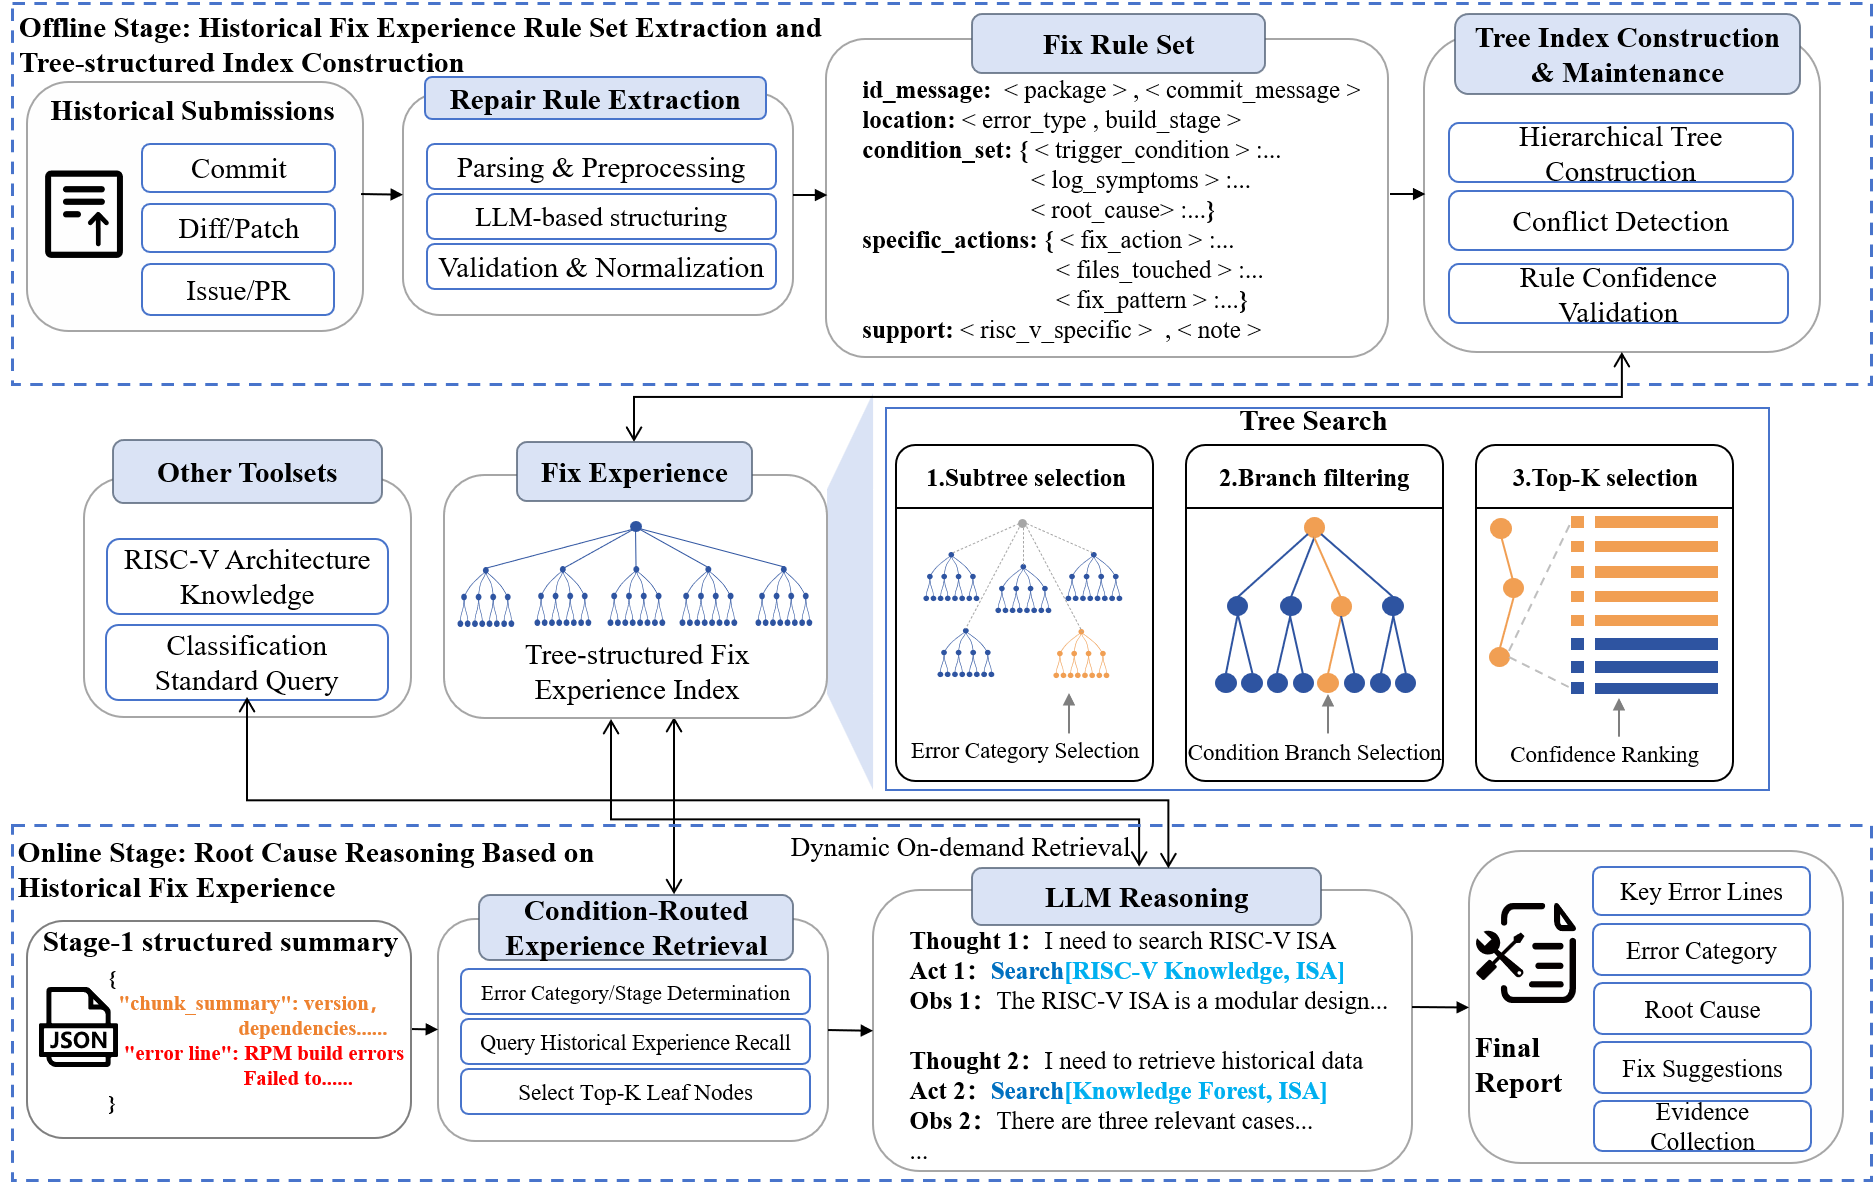
\includegraphics[width=\textwidth]{pic/hrl-rca-overview.png}
    \caption{Unravel Stage-2: Rule-Tree Reasoning for Traceable Root-Cause Diagnosis}
    \Description{A framework diagram showing offline rule extraction from historical commits and online conditional routing over a rule tree for root cause analysis.}
    \label{fig:hrl-overview}
\end{figure*}

\subsection{Reasoning Stage: Rule-Tree Reasoning for Traceable Root-Cause Diagnosis}\label{sec:hrl}

To mitigate the similarity misleading inherent in naive similarity-based retrieval and to ensure that repair recommendations are verifiable with explicit evidence, we design Stage-2 as rule-tree-based diagnosis. The fundamental idea is to extract and explicitly structure the relationships among ``symptoms---applicability conditions---repair actions---evidence'' from historical repair records, transforming scattered experience into reusable repair rules, and to construct a maintainable rule-tree index along axes of problem category, build stage, and verifiable conditions. During online inference, rather than retrieving by similarity directly, we use the Stage-1 summary as input for conditional routing over the rule tree, activating rules only when their applicability conditions are satisfied, and subsequently generating root cause explanations and fixes under explicit evidence constraints. This paradigm yields interpretable, traceable, and actionable diagnostic outputs.

As shown in Figure~\ref{fig:hrl-overview}, the overall workflow contains an offline construction and an online inference part. Offline, we process historical repair commits to extract and structure repair experience from commit messages, diffs/patches, and packaging-related spec changes, and store them as reusable rules. Then, we construct a rule-tree skeleton organized by error category and build stage, and attach each rule to leaf nodes whose conditions are satisfied, with conflict detection and incremental updates. Online, we take the Stage-1 summary $S$ (optionally augmented with spec/patch and environment summaries) as input, first determine error type and build stage to locate the entry in the rule tree, and then traverse conditional branches to retrieve candidate leaf rules. Under evidence constraints, we finally generate a diagnostic report containing ``root cause---fix---applicability conditions---evidence references''.

\subsubsection{Structuring Historical Repair Information}

In practice, historical repair experience is primarily recorded in version-control commits, encompassing commit messages, code diffs/patches, and packaging-related spec changes. Although these artifacts contain rich repair knowledge, they are inherently unstructured, stylistically heterogeneous, and varied in evidence granularity: the same category of problem may be described in disparate terms (e.g., ``fix build'', ``riscv workaround'', ``linker error''), while the actual executable repair actions are often embedded within diff fragments. Directly using raw commits as retrieval targets in similarity-based methods readily reintroduces similarity misleading and fails to explicitly capture the relationship between applicability conditions and repair actions. Therefore, Stage-2 first abstracts historical commits into structured units---repair rules---thus elevating experience from free text to computable, routable, and maintainable knowledge items.

\begin{sloppypar}
Rule construction takes a single repair commit as the basic object, with inputs including: (1) commit message describing intent and background; (2) diffs/patches containing concrete code or script changes; (3) spec changes related to packaging (e.g., dependency declarations, macro and build-parameter modifications, patch references); and (4) associated issue/PR discussions providing information about reproduction, applicability conditions, and boundary cases. The output is a structured JSON record whose fields emphasize two aspects. First, applicability conditions are explicitly encoded (e.g., \texttt{error\_type}, \texttt{build\_stage}, \texttt{trigger\_condition}, \texttt{risc\_v\_specific}, \texttt{can\_generalize}) to support later tree construction and conditional routing. Second, evidence carriers (e.g., \texttt{files\_touched}, \texttt{commit\_id}, \texttt{notes}) are preserved to ensure traceability and human verification.
\end{sloppypar}

\begin{sloppypar}
The construction pipeline adopts a three-step process: ``traditional parsing and preprocessing---LLM-based structuring---validation and normalization''. First, we use traditional techniques to pre-parse metadata and changes, including segmenting commit messages, diffs/patches, spec changes, and associated issue/PR content, and extracting salient elements such as touched files, key change hunks, dependency declarations, and macro/parameter modifications. This reduces input noise and provides structural hints for LLMs. Second, with unified prompt templates and fixed output schemas, we invoke an LLM to convert parsed results into structured repair rules, covering fields such as \texttt{error\_type}, \texttt{build\_stage}, \texttt{trigger\_condition}, \texttt{root\_cause}, and \texttt{fix\_action}, and mapping key fields such as triggers and fix patterns to predefined label sets whenever possible. Finally, an independent validation module automatically checks LLM outputs: it verifies schema conformance (field completeness, type consistency, non-empty required fields) and performs normalization consistency checks for \texttt{fix\_action} and \texttt{trigger\_condition}. When validation fails, the system triggers a rewrite strategy, asking the model to regenerate specific fields using feedback from validation, ensuring that only rules with stable formats, routable conditions, and traceable evidence enter the knowledge base.
\end{sloppypar}

\subsubsection{Rule-Tree Index Construction and Maintenance}

After obtaining structured rules, we must organize the dispersed repair experience into a routable and maintainable knowledge structure. We adopt a tree index for knowledge organization for three reasons. First, the manual diagnostic workflow for build failures inherently follows a decision path of first determining error category and build stage, then narrowing down by applicability conditions. A tree index explicitly encodes this process as conditional branches, rendering rule-matching paths naturally interpretable and auditable. Second, the effectiveness of repair experience is strongly conditioned on prerequisites (e.g., software versions, target architecture, dependency states, build systems, and build stages). Tree routing mandates that each step satisfy verifiable conditions, filtering out inapplicable rules at the retrieval entry point and thereby mitigating the risks of erroneous retrieval due to superficial similarity. Third, supplying all rules and their conditions to an LLM for ad-hoc conditional retrieval would entail prohibitive token costs, and the model would be susceptible to attention dispersion and overlooked conditions amid the resulting redundancy. The tree index pre-materializes the routing structure, performing structural pruning prior to LLM inference and injecting only the small subset of rules that satisfy the current conditions, thus enabling compact-context, strongly constrained, and auditable reasoning.

This design is distinct from both knowledge graphs and machine-learned decision trees. Knowledge graphs (e.g., LogKG~\cite{sui2023logkg}) represent failure events as entity--relation triples suited for graph-based inference, but their edges do not directly encode executable fix actions or verifiable preconditions. Machine-learned decision trees derive splits from statistical features and produce classification labels, not actionable repair recommendations with provenance. The rule tree instead encodes the diagnostic workflow of domain experts: each root-to-leaf path mirrors the decision sequence a human engineer follows (error type $\to$ build stage $\to$ specific conditions), and leaf nodes store concrete fix actions traceable to historical commits.

As illustrated in Figure~\ref{fig:rule-tree}, we start from a root node and split the first layer into five domains in accordance with our error taxonomy (architecture compatibility, version compatibility, dependency configuration, compilation configuration, and other errors), so that online inference can first perform coarse routing at the problem-domain level. The second layer is organized by build stage (e.g., \texttt{\%prep}, \texttt{\%build}, \texttt{\%install}, \texttt{\%check}), constraining historical experience to consistent stage contexts to avoid misinterpretation of the same error text under different stages. Deeper nodes branch according to verifiable routing conditions derived from \texttt{trigger\_condition} and \texttt{log\_symptoms} in rules, such as ``whether dependency xxx is detected missing'', ``whether the failure only occurs on RISC-V'', etc. Leaf nodes store sets of concrete repair rules with their \texttt{fix\_action}, applicability conditions, and annotations. Once a path is hit during online inference, the system obtains a joint package of ``conditions---actions---evidence''.

\begin{figure}[!htbp]
    \centering
    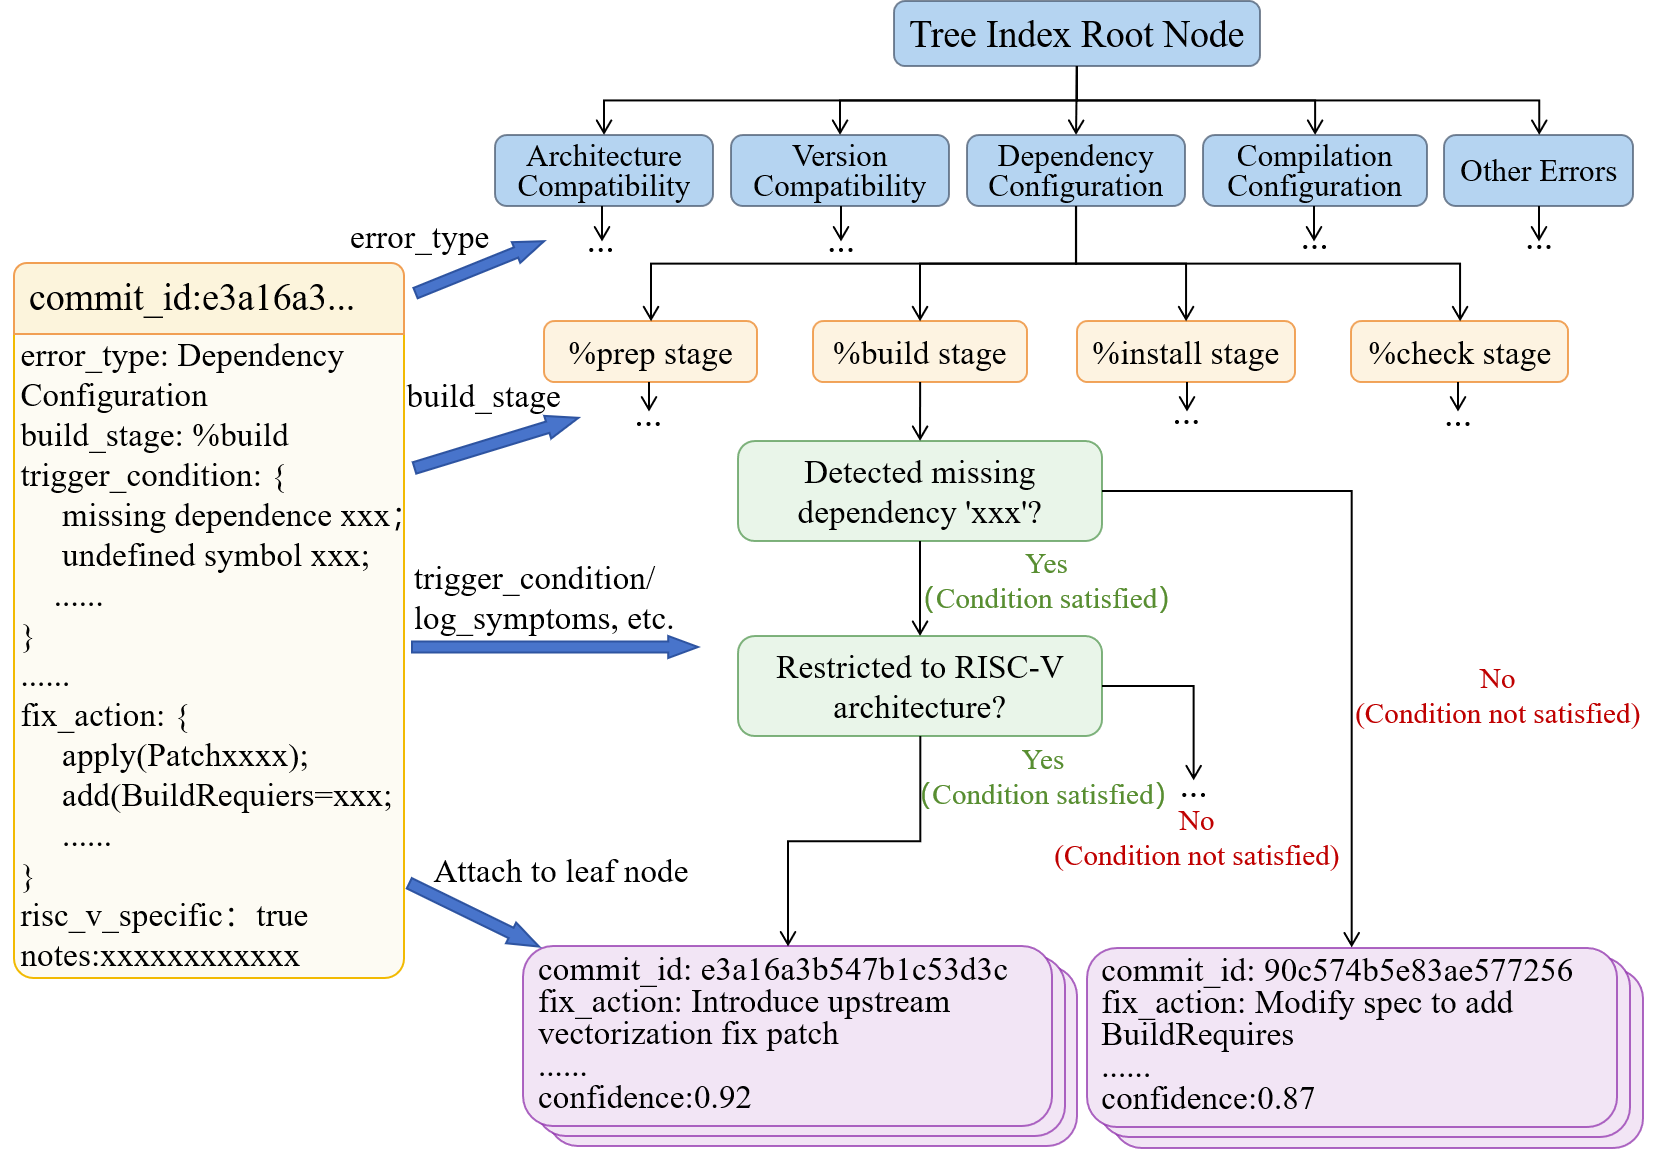
\includegraphics[width=\columnwidth]{pic/rule-tree.png}
    \caption{Illustration of the rule-tree index structure}
    \Description{A tree diagram with the root branching into five error categories, each further split by build stage, and leaf nodes storing structured repair rules.}
    \label{fig:rule-tree}
\end{figure}

To support continuous evolution, we design incremental updates and conflict-resolution mechanisms. Given a new rule, we first normalize it using the same offline procedure and then determine its routing position. If the condition set $C_{new}$ of the new rule and $C_{old}$ of an existing rule have inclusion relationships, we handle them as follows: when $C_{new} \supset C_{old}$, the new rule has stricter conditions, so we add a deeper branch in the tree and give the fine-grained rule higher priority; when $C_{new} \subset C_{old}$, the new rule is more general, and we adjust the tree to generalize conditions and reduce duplicate branches. This avoids naive stacking of rules that would lead to path explosion.

We further introduce rule confidence for quality control:
\begin{equation}
\mathrm{Conf}(r) = \alpha \cdot S_{evi}(r) + (1-\alpha) \cdot S_{time}(r)
\end{equation}
where $S_{evi}(r) = n_r / (n_r + k)$ is evidence support (with $n_r$ being the number of supporting records and $k$ a smoothing constant, default $k{=}3$), and $S_{time}(r) = 1 / (1 + (t_{now} - t_r)/T)$ measures recency (with $T{=}90$ days, meaning the recency drops to 0.5 after 90 days). Rules whose confidence falls below a threshold are used only as low-priority candidates and placed in a queue for manual review; only those above the threshold become high-priority leaf evidence for routing. This mechanism jointly constrains knowledge quality and freshness during incremental evolution.

\subsubsection{Online Root Cause Reasoning}

In the online phase, given a build-failure instance, the objective is to perform conditional routing and historical-experience retrieval along the rule tree, and then, under explicit evidence constraints, generate interpretable, actionable, and verifiable root cause analyses and repair recommendations. We adopt an iterative evidence-driven reasoning framework, employing the Stage-1 summary $S$ as the entry point and encapsulating rule-tree queries and RISC-V knowledge lookups as invocable tools. The model iterates between hypothesis formulation and evidence verification to progressively accumulate support and converge on applicable rules.

\textbf{Error type and stage determination.} In Stage-2, the first step is to determine the error category and build stage of the current failure. The Stage-1 summary $S$ already encodes explicit error lines, stage-related clues, key entities, and supporting evidence snippets. If $S$ explicitly contains stage information, we use it directly; otherwise, we infer the stage from characteristic patterns surrounding the error anchors. For error categorization, we map error anchors and entities in $S$ to one of our five predefined categories via a standardized decision procedure. When $S$ reveals architecture-specific entities or patterns, we optionally invoke RISC-V knowledge tools for supplementary verification to prevent misclassification based solely on surface-level error messages.

\textbf{Retrieving relevant historical repair experience.} After determining error type and stage, we query the rule tree. We first locate the appropriate problem-domain node according to \texttt{error\_type} and then descend into the corresponding stage subtree according to \texttt{build\_stage}, confining candidates to a semantically coherent region. Within the stage subtree, we use triggers and key entities extracted from $S$ to evaluate branch conditions. We traverse top-down: when evidence unambiguously satisfies a branch condition, we follow it; when evidence is insufficient for a definitive judgment, we retain the branch as a candidate to avoid premature pruning; when evidence explicitly contradicts a branch, we skip it. If multiple leaf nodes remain, we rank their rules by matching degree (coverage of triggers and entities) and rule confidence, retaining the Top-$K$ rules as candidate evidence. If no leaves are matched, we back off to higher-level nodes and fall back to more general rules.

\textbf{Iterative evidence-driven reasoning.} Upon retrieving candidate rules, we proceed to diagnostic output generation. Three categories of information are assembled in the LLM context: (1) the Stage-1 summary $S$, providing error anchors, stage clues, and entities; (2) retrieved historical rules (Top-$K$ candidates); and (3) routing path metadata (problem domain, stage, and branch sequence). The model first formulates preliminary hypotheses based on $S$ and the candidate rules. Crucially, the available tool set is domain-constrained: tools are limited to rule-tree queries, RISC-V ISA knowledge lookups, and applicability-condition verification, confining the reasoning trajectory within the build-failure domain and preventing hallucination-prone free-form exploration. When the model identifies missing critical information or inconsistencies among candidates, it issues ``actions'' to invoke these tools, incorporates tool outputs as ``observations,'' and then refines its hypotheses accordingly. The model is required to produce a structured diagnostic report comprising: (1) key error and stage localization; (2) error-type classification with rationale; (3) a verifiable root cause explanation; (4) concrete, executable repair recommendations; and (5) supporting evidence with references to historical repairs. When multiple candidate rules remain plausible, the system outputs a primary recommendation alongside alternatives, each annotated with its \texttt{trigger\_condition} delineating applicability boundaries, thereby avoiding unverifiable compromises when evidence conflicts.

%% ===== Section 4 Evaluation =====
\section{Evaluation}

We evaluate the proposed framework from four complementary perspectives:
\begin{itemize}[leftmargin=*]
\item \textbf{RQ1 (Extraction Effectiveness):} How well does Stage-1 preserve diagnosis-critical evidence compared with representative extraction baselines?
\item \textbf{RQ2 (Extraction Ablation):} How much does each module of Stage-1 contribute to final extraction quality?
\item \textbf{RQ3 (Diagnosis Effectiveness):} How does Unravel perform against mainstream retrieval- and search-based RCA baselines?
\item \textbf{RQ4 (Efficiency):} Can Unravel maintain practical latency while improving diagnostic quality?
\end{itemize}

\subsection{Experimental Setup}

\subsubsection{Datasets}
\begin{sloppypar}
Our experiments are conducted on real build-failure logs collected from a production OBS environment for RISC-V package migration. We use a shared dataset of 127 build-failure logs (149{,}219 lines in total) for both stages of Unravel, but evaluate them with separate protocols: Stage-1 is evaluated as an evidence-extraction task, while the full pipeline is evaluated as a root-cause-analysis task. For Stage-1 evaluation, domain experts annotate 4{,}582 repair-relevant lines as ground truth. For full-pipeline evaluation, each sample in this same 127-case dataset is evaluated as one failure case. The five RCA categories are architecture compatibility, version compatibility, dependency configuration, compilation configuration, and other errors. The Stage-1 fine-tuning dataset (2,925 examples) is collected and split independently, with no overlap with this 127-case evaluation dataset.

Figure~\ref{fig:dataset} shows that version-compatibility errors are the most frequent (40/127, 31.5\%), followed by dependency-configuration errors (35/127, 27.6\%), compilation-configuration errors (24/127, 18.9\%), other errors (17/127, 13.4\%), and architecture-compatibility errors (11/127, 8.7\%). In terms of build stages, failures are concentrated in \texttt{\%build} (59/127, 46.5\%), followed by \texttt{\%prep} (38/127, 29.9\%), \texttt{\%check} (23/127, 18.1\%), and \texttt{\%install} (7/127, 5.5\%).
\end{sloppypar}

\begin{figure}[!htbp]
    \centering
    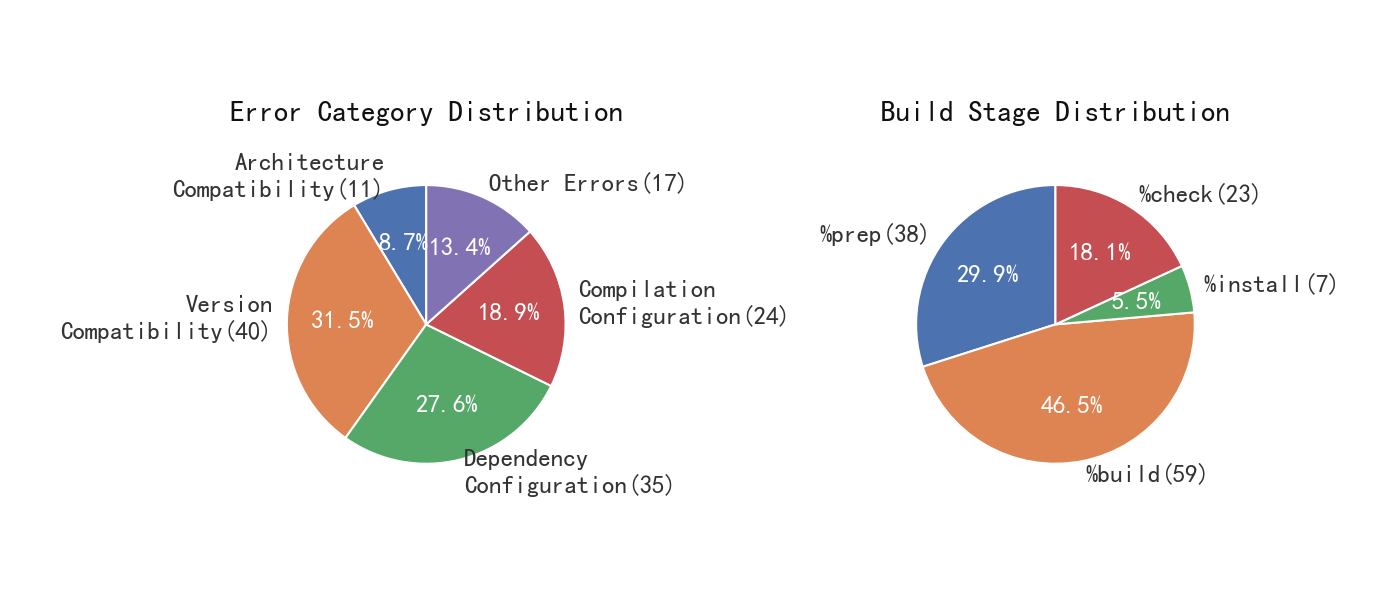
\includegraphics[width=\columnwidth]{pic/dataset-dist.png}
    \caption{Distribution of error categories and build stages in the RISC-V build-failure dataset}
    \Description{Two pie charts showing the distribution of five error categories and four build stages in the dataset.}
    \label{fig:dataset}
\end{figure}

\subsubsection{Baselines}
For evidence extraction, Unravel Stage-1 is compared with three representative baselines: (1) LogSage~\cite{xu2025logsage}, an LLM-based long-log analysis framework; (2) TemplateRAG~\cite{shuai2025root}, a template parsing plus retrieval-augmented method; and (3) LogPrompt~\cite{liu2024logprompt}, a prompt-engineering strategy for LLM-based log analysis.

For root cause analysis, we include four baseline groups: (1) naive RAG with semantic retrieval plus generation; (2) LogSage~\cite{xu2025logsage} with multi-path retrieval enhancement; (3) MCTS~\cite{shuai2025root} as a search-based reasoning framework; and (4) standalone reasoning models (Seed~1.8\footnote{Seed 1.8: \url{https://seed.bytedance.com}}, Kimi~K2\footnote{Kimi K2: \url{https://kimi.ai}}, DeepSeek-V3.2), which emphasize stronger native reasoning capability.

\subsubsection{Implementation Details}
For Unravel and comparable baselines, we use DeepSeekV3 and GPT-OSS (an open-source 120B-parameter model released by OpenAI, deployed on our infrastructure) as backbones. Standalone reasoning models are evaluated end-to-end using Stage-1 structured extraction outputs as inputs. The Stage-1 extractor is fine-tuned from Qwen3-4B-Instruct with LoRA-based parameter-efficient tuning (Section~\ref{sec:ceel}). The rule-tree knowledge base is built offline from historical OBS repair commits using the pipeline in Section~\ref{sec:hrl}.

\subsubsection{Metrics}
\begin{sloppypar}
For critical-error extraction, we report line-level Precision, Recall, and F1 to measure key-evidence preservation quality. For root cause analysis, we use the following composite score:
\begin{equation}
\text{score}(i) = \frac{s_i + c_i + r_i + f_i}{4}
\end{equation}
where $s_i$ denotes key-error extraction quality, $c_i$ error-type classification quality, $r_i$ root-cause explanation quality, and $f_i$ repair recommendation quality. Each sub-score ranges from 0 to 1 and is independently rated by three domain experts using a five-level rubric: 1.0 (fully correct), 0.75 (mostly correct with minor omissions), 0.5 (partially correct), 0.25 (mentioned but largely incorrect), and 0 (missing or incorrect). The final sub-score is determined by majority voting. Inter-annotator agreement reaches Fleiss' $\kappa=0.72$, indicating substantial consistency.
\end{sloppypar}

\subsection{RQ1: Effectiveness of Unravel Stage-1 for Evidence Extraction}

\begin{table}[htbp]
\centering
\caption{Accuracy comparison of critical-error extraction methods}
\label{tab:mgsc-results}
\begin{tabular}{lccc}
\hline
\textbf{Method} & \textbf{Prec} & \textbf{Rec} & \textbf{F1} \\
\hline
LogPrompt & 0.262 & 0.305 & 0.282 \\
TemplateRAG & 0.047 & \textbf{0.764} & 0.089 \\
LogSage & \textbf{0.314} & 0.581 & 0.408 \\
Unravel Stage-1 (ours) & 0.308 & 0.671 & \textbf{0.423} \\
\hline
\end{tabular}
\end{table}

Table~\ref{tab:mgsc-results} shows that Unravel Stage-1 achieves the best overall balance among the compared methods: it obtains the highest F1 score (0.423) while maintaining high recall (0.671). Compared with LogSage, Stage-1 improves recall by approximately 15.5\% and F1 by about 3.7\%, indicating that it preserves more key repair evidence without introducing excessive noise. TemplateRAG reaches the highest recall (0.764) but suffers from extremely low precision (0.047), suggesting heavy over-retention of irrelevant content. In contrast, Stage-1 keeps precision and recall in a more practical range for downstream diagnosis. In terms of token efficiency, Stage-1's average output lengths for three log groups are 3442/4234/5502 tokens, far smaller than TemplateRAG (38746/49883/55406), leaving substantially more context budget for Stage-2. Runtime results also show that Stage-1 provides about 2.3--3.6$\times$ acceleration over LogPrompt and TemplateRAG on ultra-long logs.

We note that the absolute F1 (0.423) reflects the stringency of line-level evaluation in logs averaging 1{,}175 lines. Expert annotations include supplementary context lines (e.g., surrounding function signatures) that aid human understanding but are not strictly required for automated diagnosis, and the extraction operates under an intentional budget constraint to leave sufficient context for Stage-2. The critical question is whether Stage-1 output retains sufficient evidence for correct downstream diagnosis---RQ3 answers this affirmatively (diagnostic score 84.0\%). Additionally, while Stage-1's precision is marginally lower than LogSage's (0.308 vs.\ 0.314), the substantial recall gain (0.671 vs.\ 0.581) is more consequential for downstream reasoning, since missing a key piece of causal evidence is costlier than including a few redundant lines.

\subsection{RQ2: Contribution of Each Stage-1 Component}

We perform an ablation study to assess the contribution of each Stage-1 component.

\begin{table}[htbp]
\centering
\caption{Ablation results of Unravel Stage-1}
\label{tab:mgsc-ablation}
\begin{tabular}{lccc}
\hline
\textbf{Configuration} & \textbf{Prec} & \textbf{Rec} & \textbf{F1} \\
\hline
Stage-1 (full) & 0.308 & 0.671 & 0.423 \\
w/o Anchor Filter & 0.274 & 0.352 & 0.308 \\
w/o Entity Backtracking & 0.292 & 0.584 & 0.389 \\
w/o Semantic Summarizer & 0.216 & 0.671 & 0.327 \\
\hline
\end{tabular}
\end{table}

The ablation results in Table~\ref{tab:mgsc-ablation} confirm that each Stage-1 component contributes to final performance. Removing the anchor filter causes the largest degradation, with recall dropping from 0.671 to 0.352 and F1 dropping from 0.423 to 0.308, which highlights the importance of early anchor-based localization. Removing entity backtracking leads to consistent declines in recall (0.584) and F1 (0.389), showing that cross-stage clue recovery is essential for maintaining evidence continuity. When the semantic summarizer is removed, recall remains unchanged (0.671), while precision decreases markedly (0.216 vs.\ 0.308), leading to a lower F1 (0.327 vs.\ 0.423). This indicates that removing the summarizer mainly retains more content and therefore does not hurt recall, but it introduces more noise and reduces output purity.

\subsection{RQ3: Comparison with Baselines on Root Cause Analysis}

\begin{table}[htbp]
\centering
\caption{Overall performance comparison on root cause analysis}
\label{tab:hrl-results}
\small
\setlength{\tabcolsep}{3pt}
\begin{tabular}{llccccc}
\hline
\textbf{Group} & \textbf{Method} & $s_i$ & $c_i$ & $r_i$ & $f_i$ & \textbf{Score} \\
\hline
\multirow{4}{*}{{\footnotesize DeepSeekV3}}
& RAG & 0.943 & 0.793 & 0.799 & 0.635 & 0.793 \\
& LogSage & 0.912 & 0.764 & 0.718 & 0.546 & 0.735 \\
& MCTS & 0.936 & 0.809 & 0.749 & 0.596 & 0.773 \\
& Unravel (ours) & \textbf{0.969} & \textbf{0.828} & \textbf{0.814} & \textbf{0.751} & \textbf{0.840} \\
\hline
\multirow{4}{*}{{\footnotesize GPT-OSS}}
& RAG & \textbf{0.915} & 0.773 & \textbf{0.851} & 0.750 & 0.822 \\
& LogSage & 0.839 & 0.726 & 0.762 & 0.638 & 0.741 \\
& MCTS & 0.913 & 0.788 & 0.819 & 0.635 & 0.789 \\
& Unravel (ours) & 0.908 & \textbf{0.789} & 0.829 & \textbf{0.794} & \textbf{0.830} \\
\hline
\multirow{3}{*}{{\footnotesize \shortstack{Standalone\\Reasoning}}}
& Seed 1.8 & 0.933 & 0.765 & 0.849 & 0.654 & 0.800 \\
& Kimi K2 & \textbf{0.959} & \textbf{0.804} & 0.854 & 0.674 & 0.822 \\
& DSV3.2 & 0.935 & 0.777 & \textbf{0.884} & \textbf{0.693} & 0.822 \\
\hline
\end{tabular}
\end{table}

Table~\ref{tab:hrl-results} shows that Unravel delivers the strongest overall RCA performance among methods using the same backbone. Under DeepSeekV3, Unravel achieves the best total score (0.840), surpassing MCTS (0.773) by about 8.7\% and RAG (0.793) by about 5.9\%. The largest gains appear in repair suggestion ($f_i=0.751$), where Unravel clearly exceeds all baselines, indicating that rule-conditioned retrieval improves the executability of generated fixes. Under GPT-OSS, the gap between Unravel (0.830) and RAG (0.822) narrows, which is expected: a stronger backbone reduces the marginal value of external knowledge structures by improving the model's intrinsic reasoning. Nevertheless, Unravel retains the best overall score and a clearer advantage on repair recommendations ($f_i$: 0.794 vs.\ 0.750), confirming that the rule tree's contribution lies primarily in producing executable fix actions grounded in historical evidence---a capability that stronger backbones do not fully substitute.

\begin{figure}[!htbp]
    \centering
    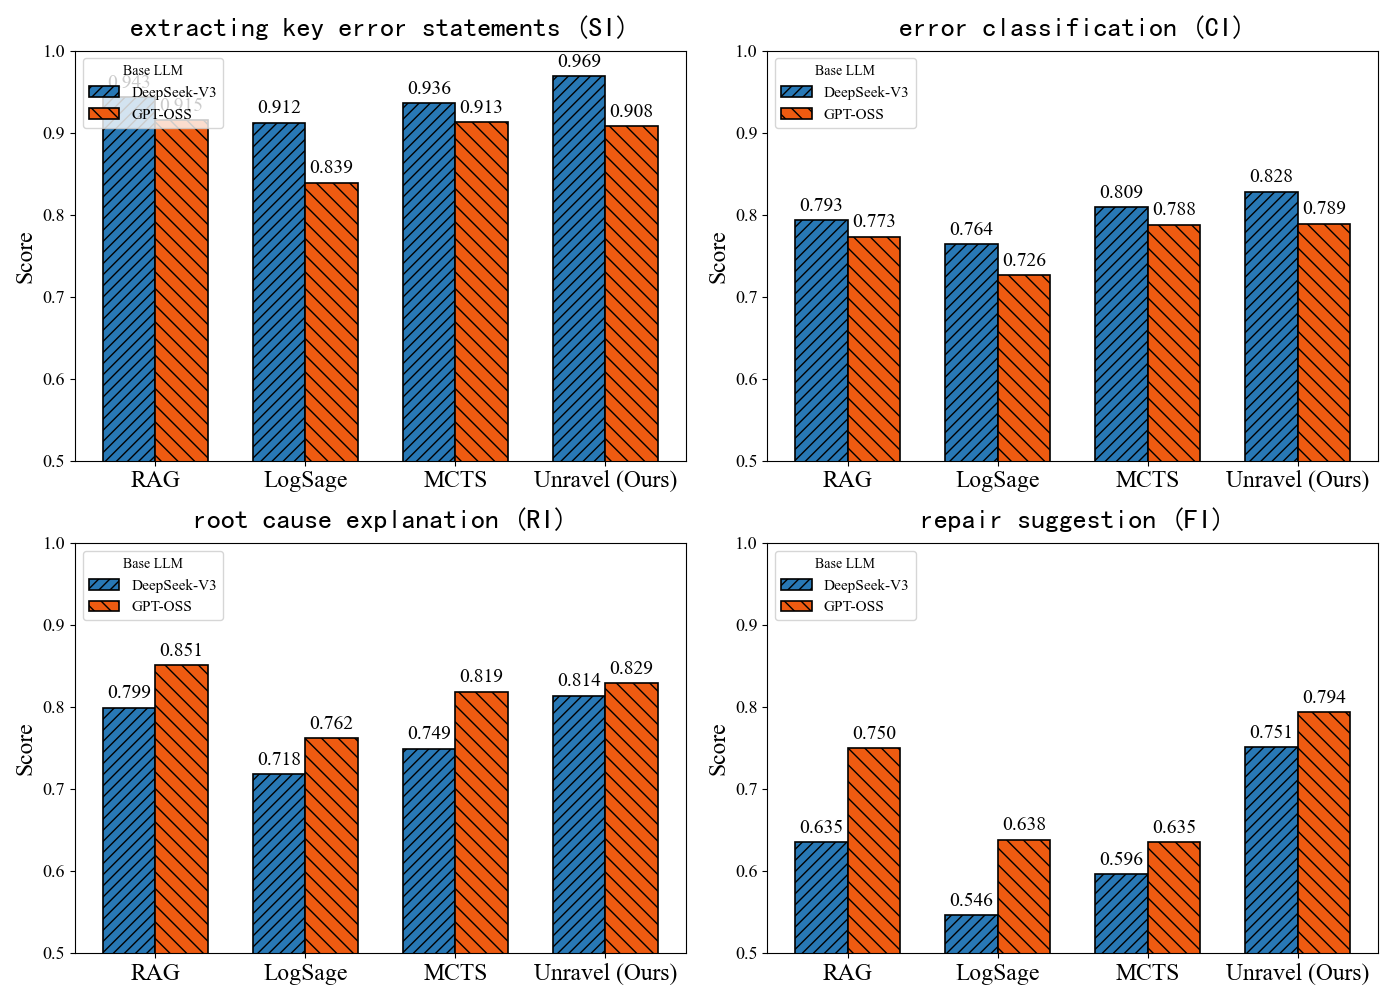
\includegraphics[width=\columnwidth]{pic/HRL-RCA-exp.png}
    \caption{Per-metric score comparison across methods}
    \Description{A grouped bar chart comparing key-error extraction, classification, root cause, and repair scores across RAG, LogSage, MCTS, and Unravel methods.}
    \label{fig:sub-scores}
\end{figure}

Figure~\ref{fig:sub-scores} further illustrates that Unravel's advantage is most pronounced in the downstream reasoning dimensions, especially repair recommendation and root cause explanation. Under DeepSeekV3, Unravel improves $f_i$ from 0.596 (MCTS) to 0.751 and raises $r_i$ to 0.814, indicating that evidence-constrained routing helps the model connect observed failures with historically validated fixes. Meanwhile, all methods obtain relatively high scores on key-error extraction, suggesting that Stage-1 already provides stable error anchors for subsequent reasoning. The remaining performance gap is therefore mainly determined by how effectively each method organizes evidence and generates actionable repair paths.

Compared with standalone reasoning models, the Unravel pipeline remains highly competitive. The best standalone scores are 0.822 (Kimi~K2 and DSV3.2), while Unravel with GPT-OSS reaches 0.830. Note that standalone models receive Stage-1 structured extraction outputs as inputs (the same as Unravel Stage-2), so this comparison isolates the contribution of rule-tree reasoning versus free-form model reasoning given identical evidence. The difference is concentrated in repair recommendations: Unravel (DeepSeekV3) achieves $f_i{=}0.751$, compared with 0.693 (DSV3.2) and 0.674 (Kimi~K2)---an 8--11\% gap. General-purpose reasoning models produce competitive root-cause explanations ($r_i$ up to 0.884) but less executable repair recommendations, because they lack access to historically validated fix patterns and their applicability conditions.

\subsection{RQ4: Efficiency Analysis}

\begin{figure}[!htbp]
    \centering
    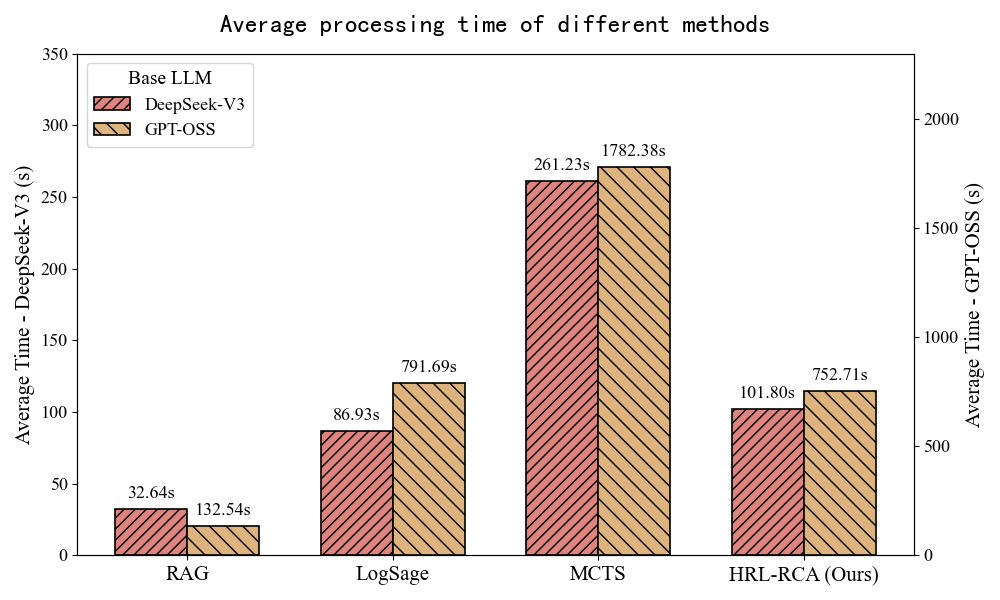
\includegraphics[width=\columnwidth]{pic/HRL-RCA-exp-time.png}
    \caption{Average processing time of different methods}
    \Description{A bar chart showing average runtime in seconds for RAG, LogSage, MCTS, and Unravel, with MCTS being the slowest and Unravel achieving a good balance.}
    \label{fig:efficiency}
\end{figure}

As shown in Figure~\ref{fig:efficiency}, Unravel achieves a favorable effectiveness-efficiency trade-off. With DeepSeekV3, its average runtime is 101.80s, which is about 61.0\% faster than MCTS (261.23s) and close to LogSage (86.93s). Although naive RAG is the fastest (32.64s), its diagnostic quality is notably lower. These results indicate that Unravel avoids the heavy cost of global search by narrowing candidates through rule routing, while retaining stronger diagnostic quality than purely retrieval-based alternatives.

\subsection{Failure Case Analysis}

To better understand residual errors, we analyze representative misdiagnosed cases and identify two major failure modes.

\textbf{(1) Incomplete complex evidence chains.} In this category, the decisive signal is a warning-triggered test failure, where interference from surrounding build/test outputs obscures the true causal path. For example, in \texttt{automake}, the key error is \nolinkurl{configure: WARNING: unrecognized options: --disable-dependency-tracking}, which should be categorized as a compilation-configuration issue. However, our method incorrectly focuses on a missing shared library (\texttt{libkmod.so.2}) in the test stage and classifies the case as a dependency-configuration problem. This case suggests that Stage-1 evidence extraction still needs stronger capability for preserving complete long-range and cross-stage evidence chains under noisy contexts.

\textbf{(2) Insufficient simulation-environment and performance knowledge.} In this category, failures are caused by memory exhaustion or timeout/deadlock effects when running tests on QEMU-based simulation environments or resource-constrained RISC-V boards. For example, in \texttt{ceph}, the actual issue is excessive parallel build jobs leading to out-of-memory behavior. Although our method correctly identifies the case as compilation configuration related, it misattributes the root cause to missing RISC-V compile flags in CMake. This indicates that Stage-2 still has notable gaps in historical repair experience and environment-aware knowledge, especially for performance-sensitive failure patterns.

%% ===== Section 5 Conclusion and Future Work =====
\section{Conclusion and Future Work}

This paper addresses build failures in RISC-V package migration by proposing Unravel, a two-stage root cause analysis framework that combines Long-Range Evidence Extraction from Build Logs with Rule-Tree Reasoning for Traceable Root-Cause Diagnosis. In Stage-1, Unravel applies rule-based error localization, entity-based cross-stage backtracking, and lightweight semantic summarization to preserve high-fidelity evidence chains under strict token budgets, substantially reducing the input size of ultra-long logs. In Stage-2, Unravel structures historical repair experience into verifiable rules organized in a rule tree and performs conditional routing during online inference to retrieve rules whose preconditions are satisfied, thereby generating traceable root cause analyses and repair recommendations under explicit evidence constraints.

Experimental results show that Stage-1 consistently improves extraction quality while preserving practical output length, reaching 0.423 F1 and improving recall and F1 over LogSage by about 15.5\% and 3.7\%, respectively. The full Unravel pipeline achieves the strongest overall RCA performance, reaching 84.0\% with DeepSeekV3 and outperforming MCTS by 8.7\% while reducing runtime by about 61.0\%. These findings demonstrate that combining evidence-preserving extraction with rule-constrained reasoning yields clear gains in both diagnostic quality and efficiency. Future work will focus on three directions: (1) improving incremental update and deduplication mechanisms for the rule knowledge base as the RISC-V ecosystem evolves; (2) extending adaptation to additional ISAs (e.g., LoongArch) and build systems (e.g., Debian, Fedora packaging); and (3) integrating the framework into CI pipelines and IDE plugins for online, developer-facing deployment. Our dataset and tools will be made publicly available upon acceptance to support reproducibility.

\section{Threats to Validity}

\textbf{Internal validity.} The RCA scoring rubric relies on expert judgment. To mitigate subjectivity, each case is independently assessed by three domain experts and the final score is determined by majority vote; the resulting Fleiss' $\kappa$ of 0.72 indicates substantial agreement. The rule-tree construction also involves LLM-based structuring, whose outputs undergo validation by an automated schema checker and a rewrite loop, thereby reducing extraction errors.

\textbf{External validity.} Our dataset is drawn from a single OBS instance focused on RISC-V. Although the 127 cases span all five error categories and four build stages---covering 20 category$\times$stage combinations with a minimum of 7 cases in the smallest cell (architecture compatibility $\times$ \texttt{\%install})---they may not fully represent all failure patterns encountered in other distributions or architectures. We note that Unravel's core algorithmic components---entity-guided backtracking, the rule-tree index structure, and iterative evidence-driven reasoning---are architecture-agnostic by design; only the regex-based filtering rules ($R_{drop}$), entity-type definitions, and the content of the rule tree are RISC-V-specific and would require re-instantiation for a new target. We plan to extend the evaluation to additional ecosystems (e.g., Debian, Fedora) and architectures (e.g., LoongArch) in future work.

\textbf{Construct validity.} The composite score equally weights four sub-dimensions. Different weighting schemes could shift relative rankings. We adopt equal weights for simplicity and report per-dimension scores in Table~\ref{tab:hrl-results} and Figure~\ref{fig:sub-scores} to allow readers to assess each dimension independently.

%%
%% Acknowledgments (hidden for submission)
%%
%\begin{acks}
%This work was supported in part by projects of the Institute of Software, Chinese Academy of Sciences, among others.
%\end{acks}

%%
%% Bibliography
%%
\bibliographystyle{ACM-Reference-Format}
\bibliography{reference}

\end{document}